%%%%%%%%%%%%%%%%%%%%%%%%%%%%%%%%%%%%%%%%%%%%%%%%%%%%%%%%%%%%%%%%%%%%%%%%
%                                                                      %
%     File: Thesis_Background.tex                                      %
%     Tex Master: Thesis.tex                                           %
%                                                                      %
%     Author: Israel Sother                                            %
%     Last modified: 27 May 2024                                       %
%                                                                      %
%%%%%%%%%%%%%%%%%%%%%%%%%%%%%%%%%%%%%%%%%%%%%%%%%%%%%%%%%%%%%%%%%%%%%%%%

\chapter{Theoretical Background and PMSM Model}
\label{chapter:background}%chktex 24

\minitoc% Creating a minitoc

This chapter covers some fundamentals used to develop this work. It starts with a brief overview of Formula Student competitions and the current powertrain system used by \gls{fst}. After this, it presents the basics on \gls{vsi} and modulation techniques before developing a mathematical model for the used motors and later converting it to discrete time. Lastly, a quick overview of the literature control methods is done before introducing the proposed strategy.
%%%%%%%%%%%%%%%%%%%%%%%%%%%%%%%%%%%%%%%%%%%%%%%%%%%%%%%%%%%%%%%%%%%%%%%%
%                                                                      %
%     File: FormulaStudent.tex           	                           %
%     Tex Master: Thesis.tex                                           %
%                                                                      %
%     Author: Israel Sother                                            %
%     Last modified: 27 May 2024                                       %
%                                                                      %
%%%%%%%%%%%%%%%%%%%%%%%%%%%%%%%%%%%%%%%%%%%%%%%%%%%%%%%%%%%%%%%%%%%%%%%%

\section{Formula Student}

In a formula student competition, two types of evaluation exist, the first category is comprised of static events where the design, cost, and business model of the prototype are analyzed. In the dynamic category, each prototype is evaluated through 5 different events: Skidpad, Acceleration, AutoX, Endurance, and Efficiency (evaluated in the Endurance track), as shown in figure \Cref{fig:fs_tracks}. To be able to compete in dynamic events each prototype needs to pass a series of safety and rule compliance inspections, a process which starts even before de competition with the documentation analysis and finishes with on-site scrutineering.

The Skidpad event is the least relevant for this study as it is designed to test the cornering ability of the vehicle. It is comprised of two circles of radius $9.125m$, where the vehicle performs an adaptation first lap and then the lap time is measured on the second lap, when the car is at steady state cornering. As it is a tight and steady course, the power consumption is low not reaching the regulations limit of $80kW$, thus the dynamic response and efficiency of the motors have almost no relevance to the performance. 

The acceleration event consists of a standing start $75m$ straight acceleration, with the maximum battery power limited to $80kw$, as it is for all Formula Student events. For this event, the key factors from a powertrain point of view are the torque dynamic response, and how efficiently the powertrain system can deliver power to the ground. 
\begin{figure}[!htb]
	\centering
	% \fbox{
	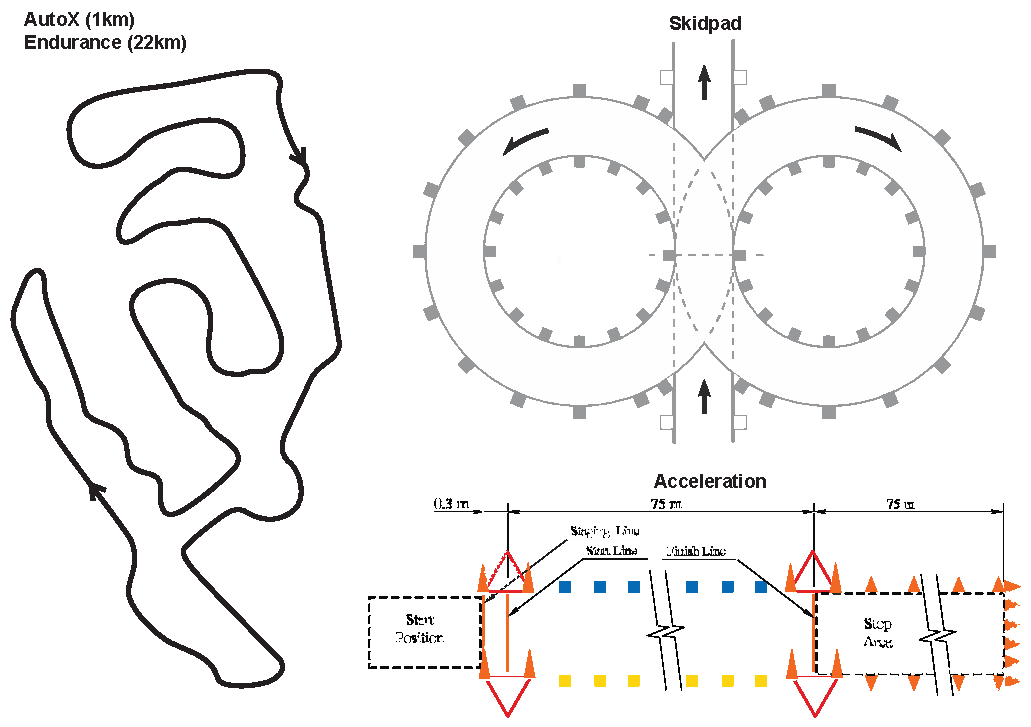
\includegraphics[width=0.8\textwidth]{Figures/Tracks.pdf}
	% }
	\caption[Formula Student Germany Tracks.]{Formula Student Germany Tracks, adapted from~\cite{FSG:rules:2023}.}
	\label{fig:fs_tracks} %chktex 24
\end{figure}
The AutoX is a $1km$ track with several corners and straights mixed. In this test, an increased dynamic response can delay the braking zone, and the efficiency allows it to reach higher velocities using the same amount of power. Lastly, the endurance event is similar to the AutoX, with enough laps to complete $22km$. In this event, although improved dynamics can be beneficial, efficiency is the key factor as it results in more available energy to complete the $22km$ track while also scoring points in the Efficiency category. 

For the autonomous part of the competition, there are very similar events, with the Skidpad and Acceleration being the same as in the manual mode. The driverless AutoX needs to be a little different, with a smaller distance for the \gls{asr} to be able to see the car throughout the entire track and press the emergency button if necessary. The Endurance event driverless analogous is the TrackDrive event, usually being on the same track as the AutoX, but with fixed 10 laps. Currently, the points performance in the driverless events is mostly dictated by how good the autonomous software is, but as the teams evolve, the cars will play a major role in the results, the same way as it is in the manual category.


Since the FST07, \gls{fst} has used AMK motors and inverters~\cite{amk:DD5-14-10-POW,amk:KW26-S5-FSE-4Q} (datasheets shown in \Cref{chapter:appendixDatasheets}), this set is a good solution for teams switching to a four-motor setup as it is already paired and has good documentation. However, as the team evolves, it is natural to look for improvements, and the AMK inverters were deemed one of the prototypes' current bottlenecks. The use of \gls{igbt} as the switching component, means that this inverter is capped in its switching frequency, using only 8kHz. This low switching frequency reduces powertrain efficiency and increases the set's weight. Another drawback of this solution is the control method as it uses a simple \gls{foc}, thus having a low dynamic response and further reducing efficiency by not using \gls{mtpa} strategies.
A brief outline of the current specification of \gls{fst}'s prototype is shown in \Cref{table:fst13_specs}.

\begin{table}[h]
	\centering
	\caption{FST13 Powertrain Specifications}
	\label{table:fst13_specs}%chktex 24
	\renewcommand{\arraystretch}{1.2} % more space between rows
	% \resizebox{0.85\textwidth}{!}{%
		\begin{tabular}{l l}
			\toprule
			% \rowcolor[HTML]{C0C0C0}
			\textbf{Parameter}                 & \textbf{Value} \\ \toprule
			Battery Voltage Min                & 420 V          \\ \hline
			Battery Voltage Maximum            & 609 V (limited at 600 V by regulations)          \\ \hline
			Battery Voltage Nominal            & 532 V          \\ \hline
			Maximum Power                      & 147 kW (limited at 80 kW by regulations)          \\ \hline
			Number of Motors                   & 4              \\ \hline
			% Motor types		                   & \gls{pmsm}\\ \hline
			% Motor Winding                      & Delta          \\ \hline
			% Motor magnet arrangement           & Spoke          \\ \hline
			Maximum Power per Motor            & 36.75 kW       \\ \hline
			Typical Average Power              & 30 kW          \\ \hline
			Maximum Average Power (1 min)      & 60 kW          \\ \hline
			Maximum Current DC                 & 160 A          \\ \hline
			Maximum motor current RMS (1,24s)  & 105 A          \\ \hline
			AMK Inverter Switching Frequency   & 8 kHz          \\ \hline
			Rotating magnetic field at Maximum Speed   & 1.6 kHz        \\ \hline
			Rated Motor Current                & 41 Arms        \\ \hline
			Rated Motor Voltage                & 350 V          \\ \hline
			% Average Current per phase          & 41             \\ \hline
			% RMS Current per phase              & 2              \\ \hline
			Maximum Speed                      & 20000 RPM      \\ \hline
			Motor Number of Poles              & 10             \\ \hline
			Quadrature Axis Inductance,        & 0.12 mH        \\ \hline
			Direct Axis Inductance             & 0.24 mH        \\ \hline
			Rotor time constant                & 0.01 s         \\ \hline
			Maximum Torque                     & 21 Nm          \\ \hline
			Torque constant                    & 0.26 Nm/Arms   \\ \hline
			Voltage constant                   & 18.8 V/kRPM    \\ \bottomrule
		\end{tabular}
	% }
\end{table}


%%%%%%%%%%%%%%%%%%%%%%%%%%%%%%%%%%%%%%%%%%%%%%%%%%%%%%%%%%%%%%%%%%%%%%%%
%                                                                      %
%     File: Inverter.tex		                                       %
%     Tex Master: Thesis.tex                                           %
%                                                                      %
%     Author: Israel Sother                                            %
%     Last modified: 27 May 2024                                       %
%                                                                      %
%%%%%%%%%%%%%%%%%%%%%%%%%%%%%%%%%%%%%%%%%%%%%%%%%%%%%%%%%%%%%%%%%%%%%%%%

\vfill
\section{Two Level Voltage Source Inverter}
\label{section:Two Level Voltage Source Inverter}%chktex 24
The usual hardware used to control synchronous machines is a 2-level Voltage Source Inverter. Such equipment is composed of six switches organized in three legs, where each pair of switches is connected to a motor terminal, as shown in \Cref{fig:inverter_and_motor_schematic}.

\begin{figure}[!htb]
	\centering
	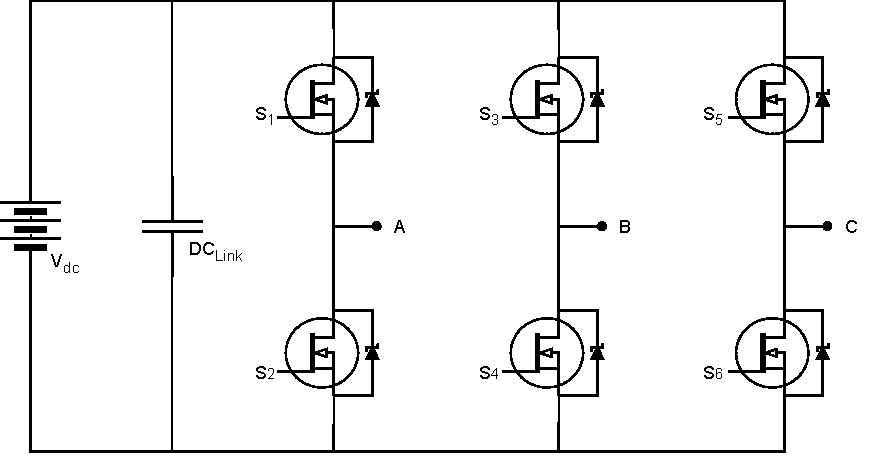
\includegraphics[width=0.7\textwidth]{Figures/Inverter.pdf}
	\caption[2-Level Voltage source Inverter arrangement.]{2-Level Voltage source Inverter arrangement.}
	\label{fig:inverter_and_motor_schematic}%chktex 24
\end{figure}

Usually, each switch in an inverter leg is operated with the inverse logic of the other switch in the leg, and this arrangement allows for 8 different switching combinations where 2 of them result in null voltages. That gives 7 possible voltage vectors, as detailed in \Cref{table:space_vector} and \Cref{fig:space_vector}. In \Cref{table:space_vector} the Vector column denotes the top switches states ($S_1$,$S_2$, and $S_3$), where a 1 means the top switch is the conducting state with the bottom switch is on a cut-off state and a 0 the opposite. The $\alpha$ and $\beta$ components which define the state space vectors are as defined by the Concordia transformation, shown in \Cref{eq:concordia}.

\begin{equation}
	\mathbf{Co} = \sqrt{\frac{2}{3}}
	\begin{bmatrix}
		1            & 0                   & \frac{1}{\sqrt{2}} \\
		-\frac{1}{2} & \frac{\sqrt{3}}{2}  & \frac{1}{\sqrt{2}} \\
		-\frac{1}{2} & -\frac{\sqrt{3}}{2} & \frac{1}{\sqrt{2}} \\
	\end{bmatrix}
	\label{eq:concordia}
\end{equation}

\begin{table}[h]
	\centering
	\caption{Switching combinations and space vectors for a 2-level three-phase inverter}
	\label{table:space_vector}%chktex 24
	\renewcommand{\arraystretch}{1.7} % more space between rows
	\resizebox{0.5\textwidth}{!}{%
		\begin{tabular}{|
				>{\columncolor[HTML]{E0E0E0}}c |
				>{\columncolor[HTML]{E0E0E0}}c |c|c|c|c|c|}
			\hline %chktex 44
			\cellcolor[HTML]{A0A0A0}\textbf{Switch State} &
			\cellcolor[HTML]{A0A0A0}\textbf{Vector}       &
			\cellcolor[HTML]{A0A0A0}\textbf{$V_{AB}$}     &
			\cellcolor[HTML]{A0A0A0}\textbf{$V_{BC}$}     &
			\cellcolor[HTML]{A0A0A0}\textbf{$V_{CA}$}	  &
			\cellcolor[HTML]{A0A0A0}\textbf{$V_{\alpha}$} &
			\cellcolor[HTML]{A0A0A0}\textbf{$V_{\beta}$}  \\ \hline %chktex 44
			0 & 000 & 0         & 0         & 0         & $0$                         & $0$                       \\ \hline %chktex 44
			1 & 001 & $V_{DC}$  & 0         & $-V_{DC}$ & $\sqrt{\frac{2}{3}}V_{DC}$  & $0$                       \\ \hline %chktex 44
			2 & 010 & $-V_{DC}$ & $V_{DC}$  & 0         & $\frac{1}{\sqrt{6}}V_{DC}$  & $\frac{1}{\sqrt{2}}V_{DC}$\\ \hline %chktex 44
			3 & 011 & 0         & $V_{DC}$  & $-V_{DC}$ & $-\frac{1}{\sqrt{6}}V_{DC}$ & $\frac{1}{\sqrt{2}}V_{DC}$\\ \hline %chktex 44
			4 & 100 & 0         & $-V_{DC}$ & $V_{DC}$  & $-\sqrt{\frac{2}{3}}V_{DC}$ & $0$                       \\ \hline %chktex 44
			5 & 101 & $V_{DC}$  & $-V_{DC}$ & 0         & $-\frac{1}{\sqrt{6}}V_{DC}$ & $\frac{1}{\sqrt{2}}V_{DC}$\\ \hline %chktex 44
			6 & 110 & $-V_{DC}$ & 0         & $V_{DC}$  & $\frac{1}{\sqrt{6}}V_{DC}$  & $\frac{1}{\sqrt{2}}V_{DC}$\\ \hline %chktex 44
			7 & 111 & 0         & 0         & 0         & $0$                         & $0$                       \\ \hline %chktex 44
		\end{tabular}%
	}
\end{table}


Despite the number of discrete voltage states, using some modulation techniques it is possible to synthesize a resultant vector if it is inside the attainable region denoted by the hexagon in \Cref{fig:space_vector}.

The current inverter used by \gls{fst} uses this structure, but the switches are silicon \glspl{igbt}, which when compared to \gls{sic} \glspl{mosfet} has a higher switching loss, leading to lower switching frequencies being used~\cite{Gurpinar:si_sic_gan_comparison:2016:IEEE}. The lower switching frequencies cause higher distortions in the current waveforms, decreasing motor efficiency. The lower switching frequency system also needs a higher capacitance on the DC Link, while the lower efficiency of silicon semiconductors requires a bigger heatsink, leading to a higher volume and mass inverter, decreasing the power density of the solution.

\subsection{Space Vector Modulation}
\label{subsection:Space Vector Modulation}%chktex 24

Several modulation techniques have been proposed in the literature like \gls{spwm}, \gls{she}~\cite{Asadzadeh:selective_harmonic_elimination:2019}, \gls{svm}~\cite{Neacsu:SVM_intro:2001:IECON}.
% , or \gls{svc}~\cite{An:space_vector_control:2016}. Some of these techniques are exclusive of multilevel inverters, like \gls{svc}~\cite{Rodriguez:svc_multilevel:2002}, while others also work for two-level inverters. 
The most common method of modulation in digital motor control is \gls{svm}, as it is a robust, easy-to-implement technique, and allows higher voltage ratio. 

% The figure "fig:space_vector" provides a visual representation of the space vector for a 2-level three-phase inverter. It shows the possible voltage states that can be applied to the motor. The phase voltages are represented in a 2D plane, with the maximum phase voltage shown by a circle. Any point within this circle is attainable without overmodulation or neutral point shift. The hexagon represents the maximum voltage that can be applied to the motor, and the vectors within the hexagon are the possible voltage states.
\Cref{fig:space_vector} shows a 2D representation of the space vector for a 2-level three-phase inverter. The basic voltage vectors (previously defined on \Cref{table:space_vector}) are shown pointing to the hexagon corners. 
% Note that they can only reach those voltages if modulation techniques that produce shifting in the neutral point (like third harmonic injection) are used.
 Connecting the basic vectors produces the hexagon of possible voltage states.

\begin{figure}[!htb]
	\centering
	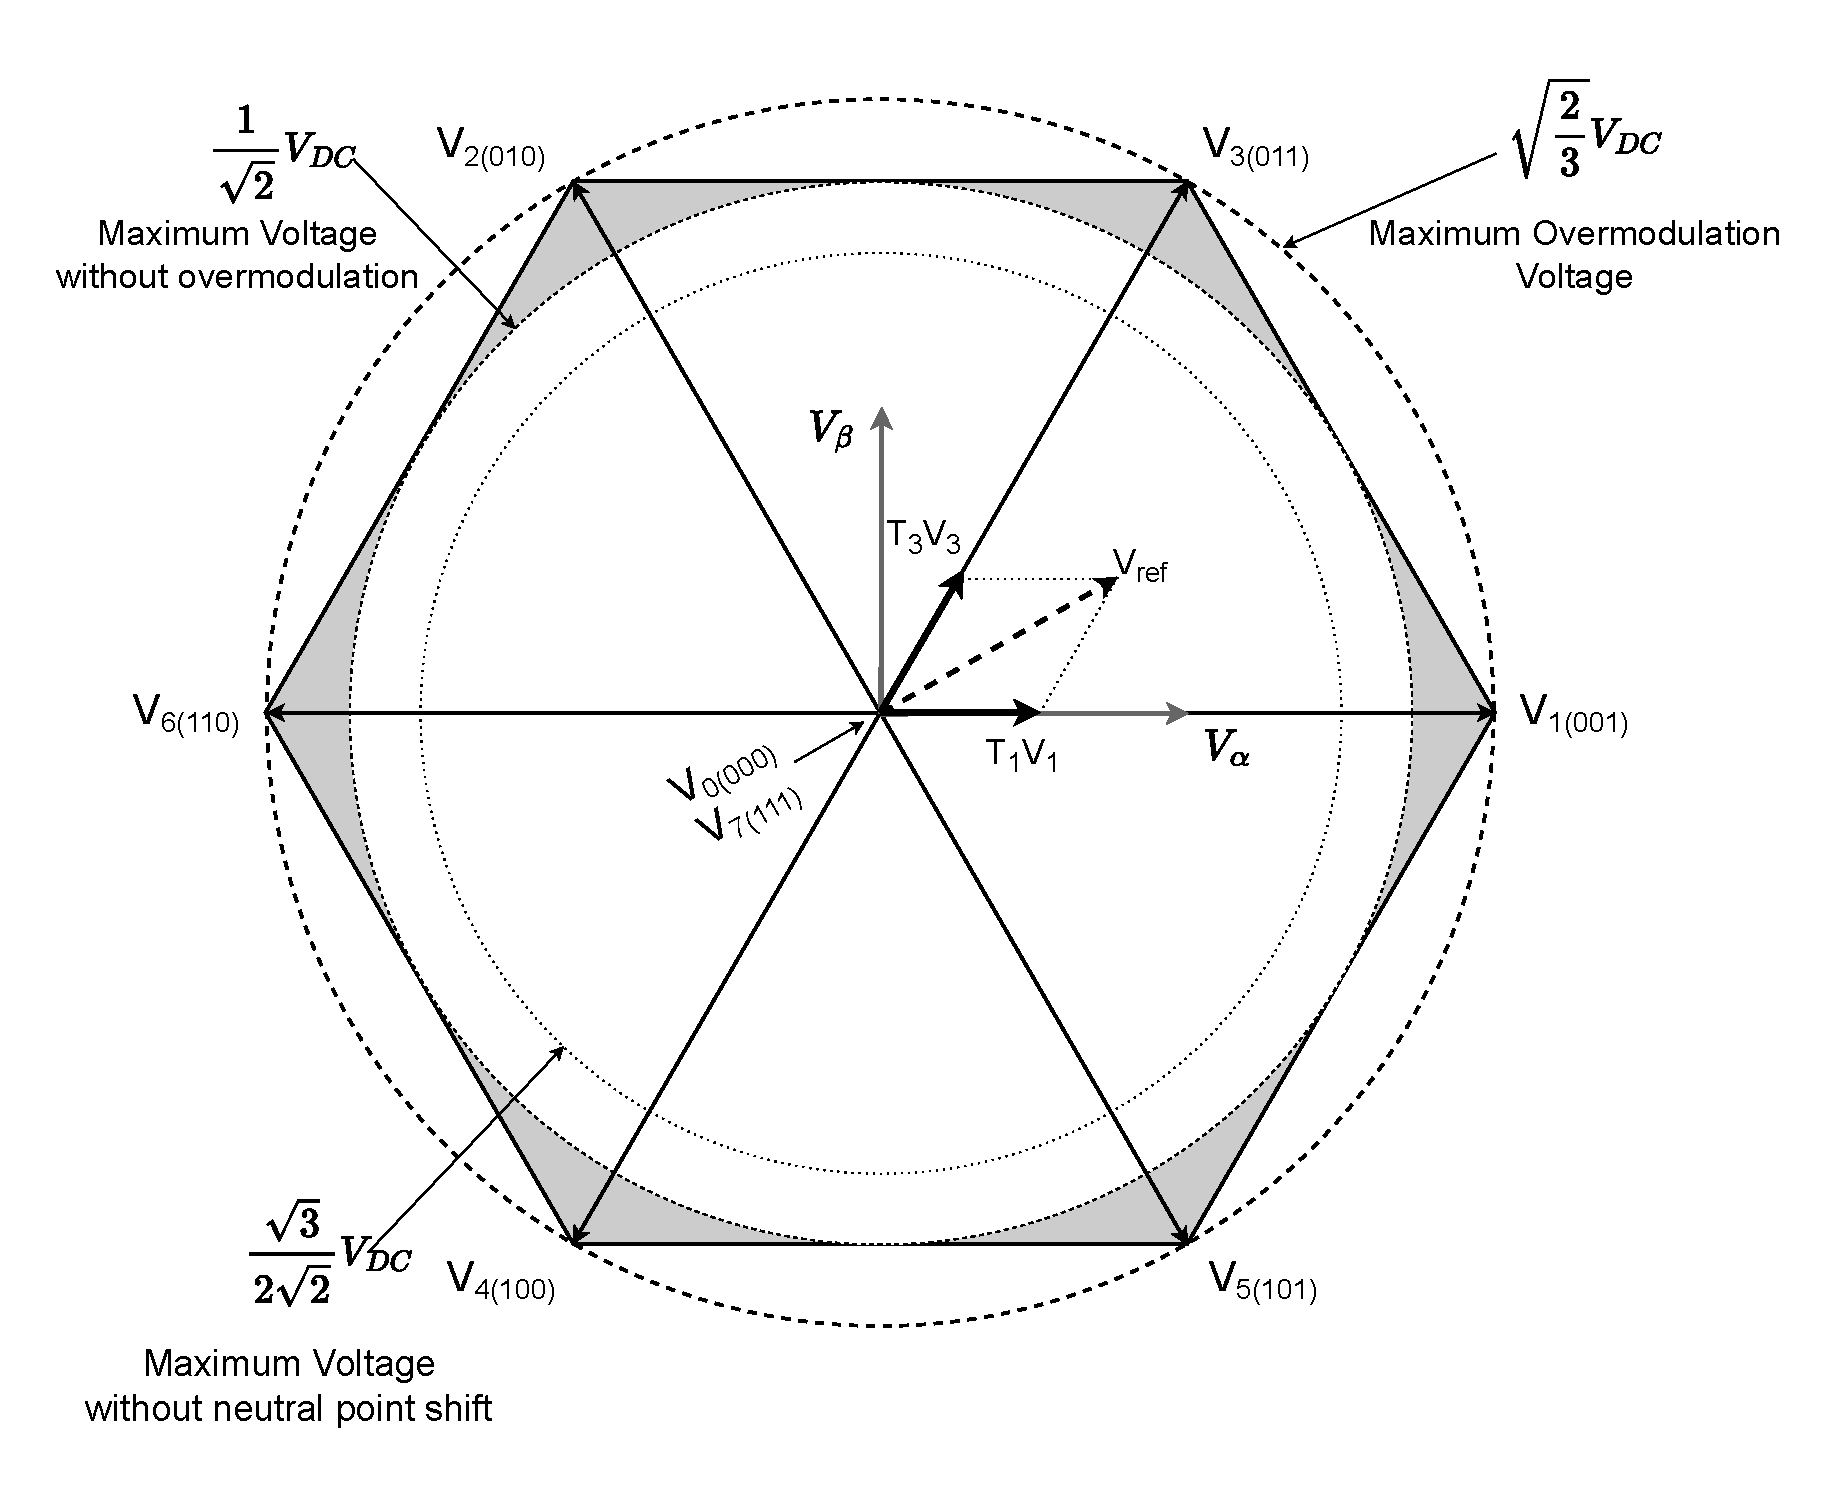
\includegraphics[width=0.8\textwidth]{Figures/Space_Vector_revised.pdf}
	\caption[Space vector for a 2-level three-phase inverter.]{Space vector for a 2-level three-phase inverter.}
	\label{fig:space_vector}%chktex 24
\end{figure}


Using \gls{svm} it is possible to modulate any vector inside the hexagon shown in \Cref{fig:space_vector}, but if a pure sinusoidal output is desired, the vectors should be constrained to the inscribed circle, that has a radius of $\frac{1}{\sqrt{2}} V_{DC}$. The reason behind this is to keep the reference vector locus inside the hexagon, avoiding distortions in the output. Note that although it is possible to generate waveforms with higher RMS value, it is not possible to modulate a peak higher than $\frac{1}{\sqrt{2}} V_{DC}$ for every vector angle. If a higher RMS value is requested the generated voltage will be saturated on the sides of the hexagon while near the corners it will achieve the requested value, thus those waveforms become more and more distorted as the amplitude approaches $\sqrt{\frac{2}{3}} V_{DC}$. To modulate a sinusoidal output the vector should develop a circular trajectory, but in the overmodulation region the voltage constrains it to the voltage hexagon, and thus the difference between the intended and the effectively applied vector increases.

To simplify the analysis of those vectors, a modulation index ($m$) is defined as shown in \Cref{eq:modulation_index}. The output is free of distortion if $m\le\frac{2}{\sqrt{3}}$, and increasing the modulation index further will result in diminishing returns in wave amplitude, while the output approaches a six-step commutation, greatly increasing the \gls{thd}~\cite{Microchip:Overmodulation:2023}. This area of operation is called overmodulation, and several approaches have been proposed~\cite{Briz:overmodulation_technique_field_weakening:2001,MehriziSani:advanced_modulation_techniques:2007} to minimize the distortions.
\begin{equation}
	m = \frac{2\sqrt{2}}{\sqrt{3}}\frac{\left|V{ref}\right|}{V_{DC}} \quad \quad m \;\in\; \left[0, \frac{4}{3}\right]
	\label{eq:modulation_index}
\end{equation}

To modulate a voltage vector that is not exactly one of the basic voltage vectors a modulation technique is needed. When using the \gls{svm} method to compose a given reference vector $V_{ref}$, the algorithm first detects the sector on which the reference vector lays. With the sector identified a ratio between the adjacent basic vectors and a null vector is selected so that the average vector is equal to the reference vector. This ratio is calculated as shown in \Cref{eq:svm_vref}.

For example, let's consider the reference vector shown in \Cref{fig:space_vector}. According to \gls{svm}, this vector can be modulated by using $V_1$ for half of the active time and $V_3$ for the other half of the active time. The active time refers to the duration when the vector amplitude is non-zero, while the null time refers to the duration when a null vector is used to reduce the output amplitude. This modulation can be expressed by \Cref{eq:svm_vref}, where $t_1+t_3$ represents the active time and $t_{n}$ represents the null time.

\begin{equation}
	V_{ref} = \frac{t_{n} V_{n} + t_1 V_1  + t_3 V_3}{h}
	\label{eq:svm_vref}
\end{equation}

%% epxplanation of the neutral point shift. it should follow the following equation: V_shift = K_{shift}*max(V_{AN},V_{BN},V_{CN) + (1-K_{shift})*min(V_{AN},V_{BN},V_{CN)


In the hardware implementation, the voltage reference is generated in the rotor reference frame (dq0) and then the inverse dq0 transformation is applied to obtain the phase voltages directly, without selecting a sector to know which vectors to use. These phase voltages are then divided by the DC link voltage to obtain the duty cycle of the switches. Note that this does not account though for the neutral point shift. This simplification results in the same switching times for the active vectors as the geometric approach of calculating which sector the reference vector is and then decomposing the reference vector in the two adjacent vectors. The null vector distribution between $V_0$ and $V_7$ will dictate the neutral point shifting method.

Several approaches have been proposed to accomplish this shift and they all rely on injecting a variable offset voltage on the neutral point that has a strong third harmonic component. Although a pure third harmonic sine wave can be used it is computationally expensive when compared with other methods such as top, mid, or bottom clamp. This technique of mid-clamp aims to center the neutral point between the DC link terminals, while the top clamp shifts the neutral point to the maximum voltage and the bottom clamp to the minimum voltage. The main advantage of a top or bottom clamp is the reduced number of switching events when compared with a mid-clamp. 

The chosen approach is defined by \Cref{eq:neutral_point_shift}, where $K_{shift}$ is the shift factor, and $V_{AN}$,$V_{BN}$, and $V_{CN}$ are the phase voltages referenced to a virtual neutral point that is the average of the phase voltages with respect to the DC link negative terminal. The value of $K_{shift}$ dictates the shift method used, when it is equal to 1 the top-clamp method is used, if it is 0.5 then the mid-clamp is used, and 0 results in the bottom-clamp method.~\citet{Microchip:ZSM_viewer:2023} has a visualization tool with the main methods shown. The calculated shift voltage is then summed to the desired phase voltages, and the modulation technique is applied as usual. In the implementation, this results in the \glspl{mosfet} duty cycle being shifted to center at the value of $K_{shift}$.

\begin{equation}
	V_{shift} = K_{shift} - K_{shift} \max \left(V_{AN},V_{BN},V_{CN}\right) - (1-K_{shift}) \min \left(V_{AN},V_{BN},V_{CN}\right)
	\label{eq:neutral_point_shift}
\end{equation}

%%%%%%%%%%%%%%%%%%%%%%%%%%%%%%%%%%%%%%%%%%%%%%%%%%%%%%%%%%%%%%%%%%%%%%%%
%                                                                      %
%     File: PMSM_model.tex                                             %
%     Tex Master: Thesis.tex                                           %
%                                                                      %
%     Author: Israel Sother                                            %
%     Last modified: 27 May 2024                                       %
%                                                                      %
%%%%%%%%%%%%%%%%%%%%%%%%%%%%%%%%%%%%%%%%%%%%%%%%%%%%%%%%%%%%%%%%%%%%%%%%
\section{PMSM model}\label{section:PMSM model}
As the proposed work is to improve the dynamic response and efficiency of the motor and motor drive currently used by \gls{fst}, it is necessary to first develop a model to represent this machine, a \gls{pmsm} with delta-arranged windings.

%%%%%%%%%%%%%%%%%%%%%%%%%%%%%%%%%%%%%%%%%%%%%%%%%%
\subsection{PMSM in ABC coordinates}
The stator voltages of the considered electrical machine can be given by \Cref{eq:flx_voltage_balance}, with a graphical representation in \Cref{fig:delta_model}.
\begin{equation}
	\begin{aligned}
		\begin{bmatrix}
			u_{AB} \\
			u_{BC} \\
			u_{CA} \\
		\end{bmatrix}
		=
		\begin{bmatrix}
			r_a & 0   & 0   \\
			0   & r_b & 0   \\
			0   & 0   & r_c \\
		\end{bmatrix}
		\begin{bmatrix}
			i_a \\
			i_b \\
			i_c \\
		\end{bmatrix}
		+
		\frac{d}{dt}
		\begin{bmatrix}
			\psi_a \\
			\psi_b \\
			\psi_c \\
		\end{bmatrix}
	\end{aligned}
	\label{eq:flx_voltage_balance}%chktex 24
\end{equation}

In this equation, $u_{xy}$ represents the measured voltage between terminal $x$ and $y$, $i_x$ is the current flowing on each phase, $r_x$ is the phase resistance, and $\psi_x$ is the flux linkage of each coil. Combining this in a matrix representation we can define the variables in \Cref{eq:variables_abc}.

\vspace{0.5cm}
\begin{subequations}
	\noindent\begin{minipage}{.38\linewidth}
		\begin{equation}
			\mathbf{R_{abc}} = \begin{bmatrix}
				r_a & 0   & 0   \\
				0   & r_b & 0   \\
				0   & 0   & r_c \\
			\end{bmatrix}
		\end{equation}
	\end{minipage}%
	\begin{minipage}{.3\linewidth}
		\begin{equation}
			\mathbf{i_{abc}} = \begin{bmatrix}
				i_a \\
				i_b \\
				i_c \\
			\end{bmatrix}
		\end{equation}
	\end{minipage}%
	\begin{minipage}{.3\linewidth}
		\begin{equation}
			\mathbf{u_{abc}} = \begin{bmatrix}
				u_{AB} \\
				u_{BC} \\
				u_{CA} \\
			\end{bmatrix}
		\end{equation}
	\end{minipage}%
	\label{eq:variables_abc}
\end{subequations}
\vspace{0.5cm}

Regarding the flux linkage, it can be defined as in \Cref{eq:flux_linkage}, where $\psi_{PM}$ is the permanent magnet flux linkage, and $\theta_e$ is the rotor electrical position. Additionally, the $L_{abc}$ matrix is the inductance matrix as later defined in \Cref{eq:phase_inductances}. With this definition, the \Cref{eq:flx_voltage_balance} can be expanded into \Cref{eq:voltage_balance}, where $E_x$ is the \gls{emf} as defined in \Cref{eq:back_emf}.

\begin{subequations}
	\noindent\begin{minipage}{.5\linewidth}
		\begin{equation}
			\pmb{\psi_{abc}} = \mathbf{L_{abc}i_{abc}} + \psi_{PM} \begin{bmatrix}
				\cos{\left(\theta_e\right)} \\
				\cos{\left(\theta_e - \frac{4\pi}{3}\right)} \\
				\cos{\left(\theta_e + \frac{4\pi}{3}\right)} \\
			\end{bmatrix}
			\label{eq:flux_linkage}
		\end{equation}
	\end{minipage}%
	\begin{minipage}{.49\linewidth}
		\begin{equation}
			\mathbf{E_{abc}} = 
			\begin{bmatrix}
				E_a \\
				E_b \\
				E_c \\
			\end{bmatrix} = \psi_{PM} \dot{\theta_e}
			 \begin{bmatrix}
				-\sin{\left(\theta_e\right)} \\
				-\sin{\left(\theta_e - \frac{4\pi}{3}\right)} \\
				-\sin{\left(\theta_e + \frac{4\pi}{3}\right)} \\
			\end{bmatrix}
			\label{eq:back_emf}
		\end{equation}
	\end{minipage}%
\end{subequations}



\begin{figure}[!htb]
	\centering
	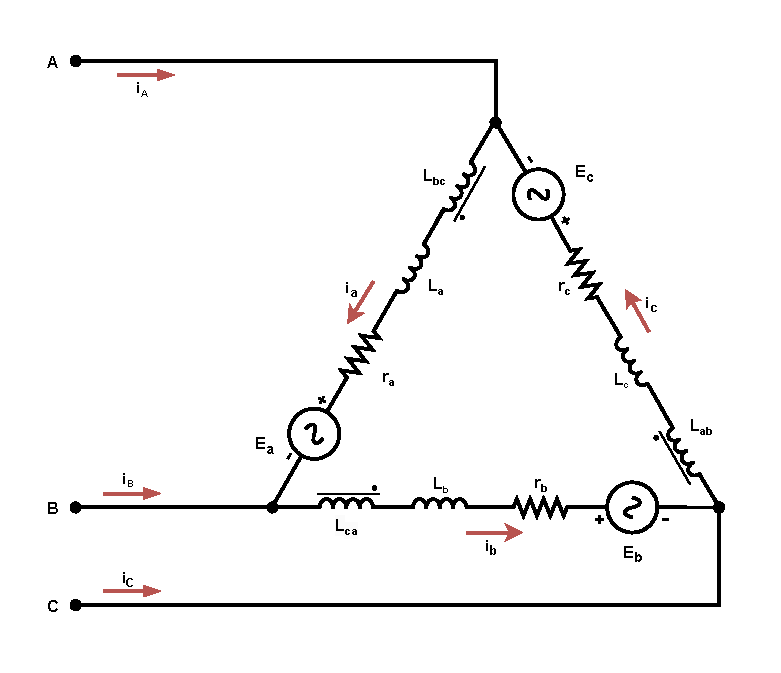
\includegraphics[width=0.6\textwidth]{Figures/Delta_model.pdf}
	\caption[Delta-wound \gls{pmsm}.]{Delta-wound \gls{pmsm}}
	\label{fig:delta_model}%chktex 24
\end{figure}
The expanded form results in~\Cref{eq:voltage_balance}.

\begin{equation}
	\mathbf{u_{abc}}
	=
	\mathbf{R_{abc}}
	\mathbf{i_{abc}}
	+
	% \begin{bmatrix}
	% 	L_{a}  & M_{ab} & M_{ac} \\
	% 	M_{ba} & L_{b}  & M_{bc} \\
	% 	M_{ca} & M_{cb} & L_{c}  \\
	% \end{bmatrix}
	\mathbf{L_{abc}}
	\frac{d\mathbf{i_{abc}}}{dt}
	+
	\frac{d\mathbf{L_{abc}}}{dt}  \mathbf{i_{abc}}
	+\mathbf{E_{abc}}
	\label{eq:voltage_balance}%chktex 24
\end{equation}


% \begin{equation}
% 	E_a + E_b + E_c + r(i_a + i_b + i_c) + (\mathbf{L} - 2\mathbf{M})\left( \frac{di_a}{dt} + \frac{di_b}{dt} + \frac{di_c}{dt}\right) = 0%chktex 7
% \end{equation}
Note that the inductances are not constant, but they change regarding the rotor electrical position $\theta_e$. This variation exists because the selected machine has a spoke magnet arrangement on the rotor, thus creating magnetic paths with different reluctances depending on the rotor angle. According to~\citet{Marques:Dinamica_das_maquinas_eletricas:2002}, this variation is a sum of even harmonics of a cosine function, but usually, it is enough to consider up to the second one, resulting in the inductance matrix shown in~\Cref{eq:phase_inductances}, where $L_{x_1}$,$L_{x_2}$,$M_{xy_1}$, and $M_{xy_2}$ are constants and define the coefficients for the self inductances and the mutual inductances.

\begin{equation}
	\mathbf{L_{abc}} =
	\begin{bmatrix}
		L_{a_1} + L_{a_2} \cos{ \left(2 \theta_e\right)}                    & M_{ab_1} + M_{ab_2} \cos{ \left(2 \theta_e + \frac{4\pi}{3}\right)} & M_{ac_1} + M_{ac_2} \cos{ \left(2 \theta_e - \frac{4\pi}{3}\right)} \\
		M_{ba_1} + M_{ba_2} \cos{ \left(2 \theta_e + \frac{4\pi}{3}\right)} & L_{b_1} + L_{b_2} \cos{ \left(2 \theta_e - \frac{4\pi}{3}\right)}   & M_{bc_1} + M_{bc_2} \cos{ \left(2 \theta_e\right)}                  \\
		M_{ca_1} + M_{ca_2} \cos{ \left(2 \theta_e - \frac{4\pi}{3}\right)} & M_{cb_1} + M_{cb_2} \cos{ \left(2 \theta_e\right)}                  & L_{c_1} + L_{c_2} \cos{ \left(2 \theta_e + \frac{4\pi}{3}\right)}   \\
	\end{bmatrix}
	\label{eq:phase_inductances}
\end{equation}

Is important to explain that the~\Cref{eq:phase_inductances} is derived assuming the 3 phases are separated by $120$ electrical degrees and that the windings have a sinusoidal magnetomotive force distribution.

For comprehensive understanding, the self inductances $L_x$ and the mutual inductances $L_{xy}$ depicted in \Cref{fig:delta_model} are as defined in \Cref{eq:induc_figure}.

\begin{subequations}
	\noindent
	\begin{minipage}{.485\linewidth}
		\begin{equation}
			L_{ab} = M_{ab_1} + M_{ab_2} \cos{ \left(2 \theta_e + \frac{4\pi}{3}\right)}
		\end{equation}
	\end{minipage}
	\begin{minipage}{.485\linewidth}
		\begin{equation}
			L_{ac} = M_{ac_1} + M_{ac_2} \cos{ \left(2 \theta_e - \frac{4\pi}{3}\right)}
		\end{equation}
	\end{minipage}
	\\
	\begin{minipage}{.485\linewidth}
		\begin{equation}
			L_{ba} = M_{ba_1} + M_{ba_2} \cos{ \left(2 \theta_e + \frac{4\pi}{3}\right)}
		\end{equation}
	\end{minipage}
	\begin{minipage}{.485\linewidth}
		\begin{equation}
			L_{bc} = M_{bc_1} + M_{bc_2} \cos{ \left(2 \theta_e\right)}
		\end{equation}
	\end{minipage}
	\\
	\begin{minipage}{.485\linewidth}
		\begin{equation}
			L_{ca} = M_{ca_1} + M_{ca_2} \cos{ \left(2 \theta_e - \frac{4\pi}{3}\right)}
		\end{equation}
	\end{minipage}
	\begin{minipage}{.485\linewidth}
		\begin{equation}
			L_{cb} = M_{cb_1} + M_{cb_2} \cos{ \left(2 \theta_e\right)}
		\end{equation}
	\end{minipage}
	\\
	\begin{minipage}{.485\linewidth}
		\begin{equation}
			L_{a} = L_{a_1} + L_{a_2} \cos{ \left(2 \theta_e\right)}
		\end{equation}
	\end{minipage}
	\begin{minipage}{.485\linewidth}
		\begin{equation}
			L_{b} = L_{b_1} + L_{b_2} \cos{ \left(2 \theta_e\right)}
		\end{equation}
	\end{minipage}
	\\
	\begin{minipage}{.95\linewidth}
		\begin{equation}
			L_{c} = L_{c_1} + L_{c_2} \cos{ \left(2 \theta_e\right)}
		\end{equation}
	\end{minipage}
	\label{eq:induc_figure}
\end{subequations}
%%%%%%%%%%%%%%%%%%%%%%%%%%%%%%%%%%%%%%%%%%%%%%%%%%
\subsection{dq0 Transformation}
\vfill
To simplify the mathematical models, some transformations were proposed. The most common is the dq0 transformation, which is a combination of the Concordia and the Blondel-Park transformations. The Concordia transformation converts a three-phase system into an equivalent two-phase system, where the two phases are orthogonal to each other, they are called $\alpha$ and $\beta$ components. This transformation has two main versions, the amplitude invariant, and the power invariant. The power invariant version, initially presented in \Cref{eq:concordia}, is shown again in \Cref{eq:concordia1} for easier reference.

The Blondel-Park transformation is a rotating referential transformation, where the referential is synchronous with the rotor position. The transformation matrix is shown in \Cref{eq:blondel_park}. Note that throughout this work the alignment of the transformation is always the $d$ component with the phase $a$. The dq0 transformation is a combination of the Concordia transformation, and the Park referential change, it produces a biphasic equivalent system with a synchronous rotating referential. The transformation matrix is shown in \Cref{eq:dq0}.

\begin{subequations}
	% \noindent
	\begin{minipage}{.4\linewidth}
		\begin{equation}
			\mathbf{Co} = \sqrt{\frac{2}{3}}
			\begin{bmatrix}
				1            & 0                   & \frac{1}{\sqrt{2}} \\
				-\frac{1}{2} & \frac{\sqrt{3}}{2}  & \frac{1}{\sqrt{2}} \\
				-\frac{1}{2} & -\frac{\sqrt{3}}{2} & \frac{1}{\sqrt{2}} \\
			\end{bmatrix}
			\label{eq:concordia1}
		\end{equation}
	\end{minipage}
	\begin{minipage}{.485\linewidth}
		\begin{equation}
			\mathbf{Bl}_{(\theta_e)} = 	\begin{bmatrix}
				\cos{\left(\theta_e\right)} & -\sin{\left(\theta_e\right)} & 0 \\
				\sin{\left(\theta_e\right)} & \cos{\left(\theta_e\right)}  & 0 \\
				0                           & 0                            & 1 \\
			\end{bmatrix}
			\label{eq:blondel_park}
		\end{equation}
	\end{minipage}
\end{subequations}
\begin{equation}
	\mathbf{T}_{(\theta_e)} = \mathbf{Co} \; \mathbf{Bl}_{(\theta_e)}
	=
	\sqrt{\frac{2}{3}}
	\begin{bmatrix}
		\cos{\left(\theta_e\right)}                & -\sin{\left(\theta_e\right)}                & \frac{1}{\sqrt{2}} \\
		\cos{\left(\theta_e-\frac{2\pi}{3}\right)} & -\sin{\left(\theta_e-\frac{2\pi}{3}\right)} & \frac{1}{\sqrt{2}} \\
		\cos{\left(\theta_e-\frac{4\pi}{3}\right)} & -\sin{\left(\theta_e-\frac{4\pi}{3}\right)} & \frac{1}{\sqrt{2}} \\
	\end{bmatrix}
	\label{eq:dq0}
\end{equation}

The power invariant transformation has the advantage of being an orthogonal matrix, thus $\mathbf{T}^{-1} = \mathbf{T}^T$.\\
If the amplitude invariant form is used, as in \Cref{eq:blondel_park_amplitude_invariant}, then orthogonality is lost.

\begin{subequations}
	% \begin{minipage}{.45\linewidth}
	\begin{equation}
		\mathbf{T}^*_{(\theta_e)} =
		\begin{bmatrix}
			\cos{\left(\theta_e\right)}                & -\sin{\left(\theta_e\right)}                & 1 \\
			\cos{\left(\theta_e-\frac{2\pi}{3}\right)} & -\sin{\left(\theta_e-\frac{2\pi}{3}\right)} & 1 \\
			\cos{\left(\theta_e-\frac{4\pi}{3}\right)} & -\sin{\left(\theta_e-\frac{4\pi}{3}\right)} & 1 \\
		\end{bmatrix}
	\end{equation}
	% \end{minipage}%
	% \begin{minipage}{.55\linewidth}
	\begin{equation}
		{\mathbf{T}^*_{(\theta_e)}}^{-1} = \frac{2}{3}
		\begin{bmatrix}
			\cos{\left(\theta_e\right)}  & \cos{\left(\theta_e-\frac{2\pi}{3}\right)}  & \cos{\left(\theta_e-\frac{4\pi}{3}\right)}  \\
			-\sin{\left(\theta_e\right)} & -\sin{\left(\theta_e-\frac{2\pi}{3}\right)} & -\sin{\left(\theta_e-\frac{4\pi}{3}\right)} \\
			\frac{1}{2}                  & \frac{1}{2}                                 & \frac{1}{2}                                 \\
		\end{bmatrix}
	\end{equation}
	\label{eq:blondel_park_amplitude_invariant}%chktex 24
	% \end{minipage}%
\end{subequations}

Applying the power invariant transformation to the abc variables results in \Cref{eq:variables_dq0}.

\begin{subequations}
	\noindent
	\begin{minipage}{.5\linewidth}
		\begin{equation}
			\mathbf{R_{dq0}} = \mathbf{T}^T_{(\theta_e)} \mathbf{R_{abc}}\mathbf{T}_{(\theta_e)}
		\end{equation}
	\end{minipage}%
	\begin{minipage}{.5\linewidth}
		\begin{equation}
			\mathbf{L_{dq0}} = \mathbf{T}^T_{(\theta_e)} \mathbf{L_{abc}}\mathbf{T}_{(\theta_e)}
		\end{equation}
	\end{minipage}%
	\\
	\begin{minipage}{.33\linewidth}
		\begin{equation}
			\mathbf{i_{abc}} = \mathbf{T}_{(\theta_e)} \mathbf{i_{dq0}}
		\end{equation}
	\end{minipage}%
	\begin{minipage}{.33\linewidth}
		\begin{equation}
			\mathbf{u_{dq0}} = \mathbf{T}^T_{(\theta_e)} \mathbf{u_{abc}}
		\end{equation}
	\end{minipage}%
	\begin{minipage}{.33\linewidth}
		\begin{equation}
			\pmb{\psi_{abc}} = \mathbf{T}_{(\theta_e)} \pmb{\psi_{dq0}}
		\end{equation}
	\end{minipage}%
	\label{eq:variables_dq0}
\end{subequations}

% Or, using the amplitude invariant form:

% \begin{subequations}
% 	\noindent
% 	\begin{minipage}{.5\linewidth}
% 		\begin{equation}
% 			\mathbf{R_{dq0}} = {\mathbf{T}^*_{(\theta_e)}}^{-1} \mathbf{R_{abc}}\mathbf{T}^*_{(\theta_e)}
% 		\end{equation}
% 	\end{minipage}%
% 	\begin{minipage}{.5\linewidth}
% 		\begin{equation}
% 			\mathbf{L_{dq0}} ={\mathbf{T}^*_{(\theta_e)}}^{-1} \mathbf{L_{abc}}\mathbf{T}^*_{(\theta_e)}
% 		\end{equation}
% 	\end{minipage}%
% 	\\
% 	\begin{minipage}{.33\linewidth}
% 		\begin{equation}
% 			\mathbf{i_{abc}} = \mathbf{T}^*_{(\theta_e)} \mathbf{i_{dq0}}
% 		\end{equation}
% 	\end{minipage}%
% 	\begin{minipage}{.33\linewidth}
% 		\begin{equation}
% 			\mathbf{u_{dq0}} = {\mathbf{T}^*_{(\theta_e)}}^{-1} \mathbf{u_{abc}}
% 		\end{equation}
% 	\end{minipage}%
% 	\begin{minipage}{.33\linewidth}
% 		\begin{equation}
% 			\pmb{\psi_{abc}} = \mathbf{T}^*_{(\theta_e)} \pmb{\psi_{dq0}}
% 		\end{equation}
% 	\end{minipage}%
% 	\label{eq:variables_dq0_amplitude}
% \end{subequations}


%%%%%%%%%%%%%%%%%%%%%%%%%%%%%%%%%%%%%%%%%%%%%%%%%%
\subsection{PMSM in dq0 coordinates}

Assuming the three phases are well balanced and using the dq0 transformation (power invariant form) to transform the model into a two-phase system with a rotating referential, new resistance and inductance matrices can be computed to this new referential. The new matrices are shown in \Cref{eq:inductance_and_resistance_dqd0}, with the subscripts $_d$, $_q$,$_0$, denoting the direct axis, the quadrature axis, and the zero-sequence axis, respectively. The transformation of the matrices is detailed in~\citet{Marques:Dinamica_das_maquinas_eletricas:2002}.

\vspace{0.5cm}
\begin{subequations}
	\begin{minipage}{.53\linewidth}
		\begin{equation}
            \mathbf{R_{dq0}} =
            \begin{bmatrix}
                r_a & 0   & 0   \\
                0   & r_b & 0   \\
                0   & 0   & r_c \\
            \end{bmatrix} =
            \begin{bmatrix}
                r & 0 & 0 \\
                0 & r & 0 \\
                0 & 0 & r \\
            \end{bmatrix}
		\end{equation}
	\end{minipage}%
	\begin{minipage}{.43\linewidth}
		\begin{equation}
            \mathbf{L_{dq0}} =
            \begin{bmatrix}
                L_d & 0   & 0   \\
                0   & L_q & 0   \\
                0   & 0   & L_0 \\
            \end{bmatrix}
		\end{equation}
    \end{minipage}
	\label{eq:inductance_and_resistance_dqd0}
\end{subequations}
\vspace{0.5cm}

Starting with \Cref{eq:flx_voltage_balance} and replacing the currents and flux linkages by their dq0 components results in \Cref{eq:voltage_balance_dq0_intermediary}.

\begin{equation}
	\begin{aligned}
		\mathbf{u_{abc}}
		=
		\mathbf{R_{abc}}
		\mathbf{T}_{(\theta_e)} \mathbf{i_{dq0}}
		+
		\frac{d\left(\mathbf{T}_{(\theta_e)} \pmb{\psi_{dq0}}\right)}{dt}
		\\
		=
		\mathbf{R_{abc}}
		\mathbf{T}_{(\theta_e)} \mathbf{i_{dq0}}
		+\dot{\theta}_e\frac{d\mathbf{T}_{(\theta_e)}}{d\theta_e}\pmb{\psi_{dq0}}
		+\mathbf{T}_{(\theta_e)}\frac{d \pmb{\psi_{dq0}}}{dt}
	\end{aligned}
	\label{eq:voltage_balance_dq0_intermediary}
\end{equation}
Replacing $\dot{\theta}_e$ with $\omega_e$, and multiplying $\mathbf{T}^T_{(\theta_e)}$ to the left yields \Cref{eq:voltage_balance_dq0_intermediary2}.
\begin{equation}
	\begin{aligned}
		\mathbf{u_{dq0}}
		=
		\mathbf{R_{dq0}}\mathbf{i_{dq0}}
		+\mathbf{T}^T_{(\theta_e)}\omega_e\frac{d\mathbf{T}_{(\theta_e)}}{d\theta_e}\pmb{\psi_{dq0}}
		+\mathbf{T}^T_{(\theta_e)}\mathbf{T}_{(\theta_e)}\frac{d \pmb{\psi_{dq0}}}{dt}
	\end{aligned}
	\label{eq:voltage_balance_dq0_intermediary2}
\end{equation}
As the transformation matrix is orthogonal, it can be further simplified, as in \Cref{eq:voltage_balance_dq0_intermediary3}.
\begin{equation}
	\begin{aligned}
		\mathbf{u_{dq0}}
		=
		\mathbf{R_{dq0}}\mathbf{i_{dq0}}
		+\omega_e\mathbf{T}^T_{(\theta_e)}\frac{d\mathbf{T}_{(\theta_e)}}{d\theta_e}\pmb{\psi_{dq0}}
		+\frac{d \pmb{\psi_{dq0}}}{dt}
	\end{aligned}
	\label{eq:voltage_balance_dq0_intermediary3}
\end{equation}
Lastly, calculate the derivative of the transformation matrix, as in \Cref{eq:transformation_derivative_intermediary,eq:transformation_derivative}.
\begin{equation}
	\label{eq:transformation_derivative_intermediary}
	\mathbf{T}^T_{(\theta_e)}\frac{d\mathbf{T}_{(\theta_e)}}{d\theta_e} = 	\frac{2}{3}
	\begin{bmatrix}
		\cos{\left(\theta_e\right)}  & \cos{\left(\theta_e-\frac{2\pi}{3}\right)}  & \cos{\left(\theta_e-\frac{4\pi}{3}\right)}  \\
		-\sin{\left(\theta_e\right)} & -\sin{\left(\theta_e-\frac{2\pi}{3}\right)} & -\sin{\left(\theta_e-\frac{4\pi}{3}\right)} \\
		\frac{1}{\sqrt{2}}           & \frac{1}{\sqrt{2}}                          & \frac{1}{\sqrt{2}}                          \\
	\end{bmatrix}
	\begin{bmatrix}
		-\sin{\left(\theta_e\right)}                & -\cos{\left(\theta_e\right)}                & 0 \\
		-\sin{\left(\theta_e-\frac{2\pi}{3}\right)} & -\cos{\left(\theta_e-\frac{2\pi}{3}\right)} & 0 \\
		-\sin{\left(\theta_e-\frac{4\pi}{3}\right)} & -\cos{\left(\theta_e-\frac{4\pi}{3}\right)} & 0 \\
	\end{bmatrix}
\end{equation}
\begin{equation}
	\label{eq:transformation_derivative}
	\mathbf{T}^T_{(\theta_e)}\frac{d\mathbf{T}_{(\theta_e)}}{d\theta_e} =
	\begin{bmatrix}
		0 & -1 & 0 \\
		1 & 0  & 0 \\
		0 & 0  & 0 \\
	\end{bmatrix}
\end{equation}
Thus, the \gls{pmsm} model in the dq0 frame is presented in \Cref{eq:flx_voltage_balance_dq0}. This approach can be used for the amplitude invariant transformation and will result in the same form of equation (\Cref{chapter:appendixdq0_amplitude}), but the equation will be scaled by a factor of $\sqrt{\frac{3}{2}}$ in the d and q axis, while the zero axis can give different results.
\begin{equation}
	\mathbf{u_{dq0}}
	=
	\mathbf{R_{dq0}}\mathbf{i_{dq0}}
	+\omega_e	\begin{bmatrix}
		0 & -1 & 0 \\
		1 & 0  & 0 \\
		0 & 0  & 0 \\
	\end{bmatrix}
	\pmb{\psi_{dq0}}
	+\frac{d \pmb{\psi_{dq0}}}{dt}
	\label{eq:flx_voltage_balance_dq0}
\end{equation}

Is worth noticing that because this is a delta wound machine, the sum of the phase currents is not necessarily zero, and as such, it is mathematically possible to have a circulating current through the phases~\cite{Pramod:circulating_currents_delta_winding:2023}, thus the zero-sequence component is not directly zero as in a Y wound device. For such currents to exist, an external exciting winding, a relevant non-considered inductance harmonic, or an imbalance through the phases is necessary. Even when those currents are present, they are usually dependent on the rotor position, and cannot be controlled with the standard 3-terminal connection,
% \textbf{REFERENCE HERE}. Some studies have shown that the zero-sequence current component is relatively small compared to the direct and quadrature ones \textbf{REFERENCE HERE}, and
thus for the sake of simplicity, they are discarded throughout this work, which gives \Cref{eq:motor_blondel_park}.
\begin{subequations}
	\begin{equation}
		u_d = r i_d+\frac{d\psi_d}{dt} - \omega_e \psi_q\\
		\label{eq:motor_blondel_park_d} %chktex 24
	\end{equation}
	\begin{equation}
		u_q = r i_q+\frac{d\psi_q}{dt} + \omega_e \psi_d\\
		\label{eq:motor_blondel_park_q} %chktex 24
	\end{equation}
	\begin{equation}
		T_e = p(\psi_d i_q - \psi_q i_d)\\
	\end{equation}
	\begin{equation}
		\frac{d\omega_e}{dt} = \frac{T_e-T_{load} - T_{loss}}{J}\\
	\end{equation}
	\begin{equation}
		\frac{d\theta_e}{dt} = \omega_e
	\end{equation}
	\label{eq:motor_blondel_park} %chktex 24
\end{subequations}

Here $\omega_e$ is the rotor electrical rotational velocity, $p$ is the number of pole pairs, $J$ is the rotor rotational inertia, while $T_e$ is the electromagnetic torque, $T_{load}$ is the reaction torque of the load attached to the motor, and $T_{loss}$ is a torque equivalent to the losses on the motor (such as iron or friction losses).



If $\psi$ is assumed to be of form $\psi = i_x L_x + \psi_{PM_x}$ where the inductance only varies with the current and the permanent magnets flux ($\psi_{PM_x}$) is defined as constant and affecting only the direct axis ($\psi_{PM_q} = 0$), \Cref{eq:motor_blondel_park_d,eq:motor_blondel_park_q} result in \Cref{eq:motor_with_inductances}.

\begin{subequations}
	\begin{equation}
		% \left\{
		% \begin{aligned}
		u_d = r i_d+\frac{d i_d}{dt}\left(L_d + i_d\frac{d L_d}{di_d}\right) - \omega_e L_q i_q                \\
	\end{equation}
	\begin{equation}
		u_q = r i_q+ \frac{d i_q}{dt} \left(L_q + i_q\frac{d L_q}{di_q}\right) + \omega_e (L_d i_d +\psi_{PM}) \\
		% T_e  = p\, i_q(( L_d - L_q)i_d + \psi_{PM})                                                              \\ %= p( (L_d i_d + \psi_{PM}) i_q - L_q i_q i_d)\\
		% \frac{d\omega_e}{dt} = \frac{T_e-T_{load} - T_{loss}}{J}                                                 \\
		% \frac{d\theta_e}{dt} = \omega_e
		% \end{aligned}
		% \right.
	\end{equation}
	\label{eq:motor_with_inductances}
\end{subequations}
Note that in \Cref{eq:motor_with_inductances} the cross-magnetization effect is not accounted for, but the saturation is included in the inductance variation~\cite{Ohm:saturation_inductance:2000}.
If the inductance derivative is small when compared with the other terms, it can be further simplified to \Cref{eq:motor_with_inductances_no_derivative}.
\begin{subequations}
	\begin{equation}
		% \left\{
		% \begin{aligned}
		u_d = r i_d+L_d\frac{d i_d}{dt} - \omega_e L_q i_q              \\
	\end{equation}
	\begin{equation}
		u_q = r i_q+L_q\frac{d i_q}{dt} + \omega_e (L_d i_d +\psi_{PM})
	\end{equation}
	\begin{equation}
		T_e  = p\, i_q(( L_d - L_q)i_d + \psi_{PM})                       \\ %= p( (L_d i_d + \psi_{PM}) i_q - L_q i_q i_d)
	\end{equation}
	\begin{equation}
		\frac{d\omega_e}{dt} = \frac{T_e-T_{load} - T_{loss}}{J}
	\end{equation}
	\begin{equation}
		\frac{d\theta_e}{dt} = \omega_e
		% \end{aligned}
		% \right.
	\end{equation}
	\label{eq:motor_with_inductances_no_derivative}
\end{subequations}

Lastly, for the sake of completeness, if the amplitude invariant dq0 transformation is used, the currents need to be multiplied by a factor of $\sqrt{\frac{3}{2}}$ in the torque equation to have a power conservative output, resulting in~\Cref{eq:torque_amplitude_invariant}. The $\sqrt{\frac{2}{3}}$ next to the $\psi_{PM}$ is just a reminder that the flux linkage value has a different value depending on the dq0 transformation used.
\begin{equation}
	T_e  = 1.5p\, i_q(( L_d - L_q)i_d + \sqrt{\frac{2}{3}}\psi_{PM})
	\label{eq:torque_amplitude_invariant}
\end{equation}
%%%%%%%%%%%%%%%%%%%%%%%%%%%%%%%%%%%%%%%%%%%%%%%%
\subsection{Discretization of the PMSM model}
\vfill
An approximation of the differential equations is needed to discretize the equations to be able to use the model in a discrete time control system. Two usual solutions are the Backward and the Forward Euler methods. Although simpler to compute, the Forward Euler method is prone to instabilities especially in fast systems such as power converters, in contrast with the Backward alternative that is unconditionally stable. Due to this consideration, the Euler Backward technique will be prioritized.

From \Cref{eq:motor_with_inductances_no_derivative}, knowing that the currents and voltages vary with time and that the inductances are dependent on the currents the derivatives are isolated, as shown in \Cref{eq:model_derivatives}.
\begin{subequations}
	\begin{equation}
	\frac{d i_d}{dt} = \frac{u_d - r i_d + \omega_e L_q i_q}{L_d}
	\end{equation}
	\begin{equation}
	\frac{d i_q}{dt} = \frac{u_q - r i_q - \omega_e (L_d i_d +\psi_{PM})}{L_q}
	\end{equation}
	\begin{equation}
		T_e  = p\, i_q(( L_d - L_q)i_d + \psi_{PM})
	\end{equation}
	\begin{equation}
	\frac{d\omega_e}{dt} = \frac{T_e-T_{load} - T_{loss}}{J}
	\end{equation}
	\begin{equation}
	\frac{d\theta_e}{dt} = \omega_e
	\end{equation}
	\label{eq:model_derivatives}
\end{subequations}
 
Then it is possible to discretize the system with $h$ as the sampling time, and $t = kh$. As the Backward Euler method is desired, the derivatives are approximated by \Cref{eq:backward_euler_example}, resulting in \Cref{eq:motor_with_inductances_discrete}

\begin{equation}
    \frac{dy}{dt} = \frac{y(k+1) - y(k)}{h}
	\label{eq:backward_euler_example}
\end{equation}

\begin{equation}
	\left\{
	\begin{aligned}
		\frac{i_{d(k+1)}-i_{d(k)}}{h} = \frac{u_{d(k+1)} -r i_{d(k+1)} +\omega_{e(k+1)} L_{q(i_q(k+1))} i_{q(k+1)}}{L_{d(i_d(k+1))}}               \\
		\frac{i_{q(k+1)}-i_{q(k)}}{h} = \frac{u_{q(k+1)} -r i_{q(k+1)} - \omega_{e(k+1)} (L_{d(i_d(k+1))} i_{d(k+1)} +\psi_{PM})}{L_{q(i_q(k+1))}} \\
		T_{e(k+1)}  = p\, i_{q(k+1)}(( L_{d(i_d(k+1))} - L_{q(i_q(k+1))})i_{d(k+1)} + \psi_{PM})                                                   \\
		\frac{\omega_{e(k+1)} - \omega_{e(k)}}{h} = \frac{T_{e(k+1)}-T_{load(k+1)} - T_{loss(k+1)}}{J}                                             \\
		\frac{\theta_{e(k+1)} - \theta_{e(k)}}{h} = \omega_{e(k+1)}
	\end{aligned}
	\right.
	\label{eq:motor_with_inductances_discrete}
\end{equation}

This set of equations has an algebraic loop, where the currents in $k+1$ depend on the value of $\omega_{(k+1)}$, that depends on the value of $T_{e(k+1)}$ that is defined by the currents in $k+1$. The same thing happens with the inductances, as they depend on the currents, but the currents define the value of inductance. Those problems are solved by first assuming that the inductance change due to the current change in a time step is small enough so that the inductances can be calculated using the previous time step currents ($ L_{x(i_x(k+1))} \approx L_{x(i_x(k))} $). Similarly, the rotor speed is assumed to vary little between iterations, so that $\omega_{(k+1)} \approx \omega_{(k)}$.

With those considerations, and rearranging the equations, the system can be solved iteratively, as shown in \Cref{eq:motor_backward_euler_matrix}.

% \begin{equation}
% 	\left\{
% 	\begin{aligned}
% 		i_{d(k+1)}
% 		= \frac{h(u_{d(k+1)} +\omega_{e(k)} L_{q(i_q(k))} i_{q(k+1)}) + i_{d(k)}L_{d(i_d(k))}}{hr  + L_{d(i_d(k))}}                        \\
% 		i_{q(k+1)} =
% 		\frac{h\left(u_{q(k+1)} - \omega_{e(k)} (L_{d(i_d(k))} i_{d(k+1)} +\psi_{PM})\right) + i_{q(k)} L_{q(i_q(k))}}{hr + L_{q(i_q(k))}} \\
% 		T_{e(k+1)}  = p\, i_{q(k+1)}(( L_{d(i_d(k+1))} - L_{q(i_q(k+1))})i_{d(k+1)} + \psi_{PM})                                           \\
% 		\omega_{e(k+1)} = \omega_{e(k)} + h\left(\frac{T_{e(k+1)}-T_{load(k+1)} - T_{loss(k+1)}}{J}\right)                                 \\
% 		\theta_{e(k+1)} = \theta_{e(k)} + h\omega_{e(k+1)}
% 	\end{aligned}
% 	\right.
% 	\label{eq:motor_backward_euler}
% \end{equation}

% Or, in matrix form, as shown in \Cref{eq:motor_backward_euler_matrix}.
\begin{subequations}
	\begin{equation}
		\begin{aligned}
			\begin{bmatrix}
				i_{d(k+1)} \\
				i_{q(k+1)} \\
			\end{bmatrix}
			=
			\begin{bmatrix}
				1                                                    & -h\frac{\omega_{e(k)}L_{q(i_q(k))}}{hr+L_{d(i_d(k))}} \\
				h\frac{\omega_{e(k)}L_{d(i_d(k))}}{hr+L_{q(i_q(k))}} & 1                                                     \\
			\end{bmatrix}^{-1} \\
			\left(
			\begin{bmatrix}
					\frac{L_{d(i_d(k))}}{hr+L_{d(i_d(k))}} & 0                                      \\
					0                                      & \frac{L_{q(i_q(k))}}{hr+L_{q(i_q(k))}} \\
				\end{bmatrix}
			\begin{bmatrix}
					i_{d(k)} \\
					i_{q(k)} \\
				\end{bmatrix}
			+
			\begin{bmatrix}
					\frac{h}{hr+L_{d(i_d(k))}} & 0                          \\
					0                          & \frac{h}{hr+L_{q(i_q(k))}} \\
				\end{bmatrix}
			\begin{bmatrix}
					u_{d(k+1)} \\
					u_{q(k+1)} \\
				\end{bmatrix}
			+
			\begin{bmatrix}
					0                                                 \\
					-h\frac{\omega_{e(k)}\psi_{PM}}{hr+L_{q(i_q(k))}} \\
				\end{bmatrix}
			\right)
		\end{aligned}
	\end{equation}

	\begin{equation}
		T_{e(k+1)}  = p\, i_{q(k+1)}((L_{d(i_d(k+1))} - L_{q(i_q(k+1))})i_{d(k+1)} + \psi_{PM})
	\end{equation}

	\begin{equation}
		\begin{aligned}
			\begin{bmatrix}
				\omega_{e(k+1)} \\
				\theta_{e(k+1)}
			\end{bmatrix}
			=
			\begin{bmatrix}
				1 & 0 \\
				h & 1
			\end{bmatrix}
			\begin{bmatrix}
				\omega_{e(k)} \\
				\theta_{e(k)}
			\end{bmatrix}
			+
			\frac{T_{e(k+1)}-T_{load(k+1)} - T_{loss(k+1)}}{J}
			\begin{bmatrix}
				h \\
				h^2
			\end{bmatrix}
		\end{aligned}
	\end{equation}
	\label{eq:motor_backward_euler_matrix}
\end{subequations}
%%%%%%%%%%%%%%%%%%%%%%%%%%%%%%%%%%%%%%%%%%%%%%%%%%%%%%%%%%%%%%%%%%%%%%%%
%                                                                      %
%     File: Control_methods_overview.tex                               %
%     Tex Master: Thesis.tex                                           %
%                                                                      %
%     Author: Israel Sother                                            %
%     Last modified: 27 May 2024                                       %
%                                                                      %
%%%%%%%%%%%%%%%%%%%%%%%%%%%%%%%%%%%%%%%%%%%%%%%%%%%%%%%%%%%%%%%%%%%%%%%%
\vfill
\section{Control Methods State of the Art}\label{section:control_methods}
The quest for higher efficiency and performance has pushed the development in the field of control of electrical machines, and even though several advances have been made, the main strategies in the market are still the \gls{foc} with PID current control, and \gls{dtc}. While robust and well-known, these methods cannot explore the full performance envelope of the controlled machines, and the development of more complex machines with increased dynamic response and efficiency has pushed for new control strategies. In this context, the use of \gls{mpc} has grown as a good alternative as it explicitly considers the system dynamics and constraints.

\subsection{Field Oriented Control}

For many years field oriented control has been one of the cornerstones of electrical machine control due to its simplicity and easy implementation~\cite{Doncker:Universal_FOC:1994}. This technique is based on the Blondel Park transformation, where it converts the currents and voltages from a stationary ABC reference frame into a rotating referential dq0. This allows the individual control of the motor magnetic flux and torque, which are proportional to $i_d$ and $i_q$ respectively. These currents usually are controlled using two separated PIDs, where the quadrature current reference comes from the desired motor torque and the direct current comes from the field weakening strategy. The PIDs compare the references with the measured values and output a voltage to be applied in each axis, voltages that are passed to a modulator (usually \gls{svm}) to calculate the duty cycle of each \gls{mosfet} and generate the control signals. An example of such a system is shown in \Cref{fig:example_PID}.
\begin{figure}[!htb]
	\centering
	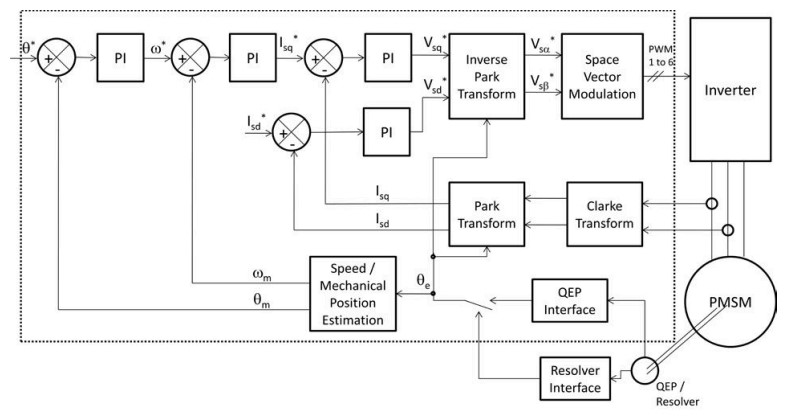
\includegraphics[width=1\textwidth]{Figures/foc_texas_instruments.jpg}
	\caption[Field Oriented Control - from Texas Instruments~\cite{TI:FOC_TMS320F2837:2016}.]{Field Oriented Control - from Texas Instruments~\cite{TI:FOC_TMS320F2837:2016}.}
	\label{fig:example_PID} %chktex 24
\end{figure}

While simple and robust, this technique heavily depends on the rotor position which is not always available, thus often needing some form of estimation to work correctly. Despite this limitation, \gls{foc} is a versatile method, being suitable not only for \gls{pmsm}, but also for induction motors, reluctance machines, among others~\cite{Hoang:FOC_vs_DTC_induction:1999,Matsuo:FOC_reluctance:1993}. One of the great advantages of \gls{foc} is that it produces a smooth operation in the full range of the motor, with low current distortions and reduced torque ripple~\cite{Adhavan:FOC_fuzzy:2011}.



\subsection{Direct Torque Control}
The principal rivel of \gls{foc} is \gls{dtc}, it shows better dynamic response with simpler implementation and less dependency on machine characterization~\cite{Hoang:FOC_vs_DTC_induction:1999}. Popularized by its use on induction machines, this method usually operates at the abc reference frame, calculating the flux based on the voltage and current vectors as in \Cref{eq:dtc_flux}, where $V_s$ is the stator voltage vector, $I_s$ is the stator current vector, $R_s$ is the stator resistance matrix, and $\psi_r$ is the rotor magnetic flux vector. Using this information, the torque can be calculated as in \Cref{eq:dtc_tq}, where $p$ is the number of pole pairs. When using an induction machine it is not necessary to have a rotor position, but on \gls{pmsm} this becomes a necessity as in \gls{foc}.

\begin{subequations}
	\begin{minipage}{.45\linewidth}
        \begin{equation}
            \psi_s = \int (V_s -R_s I_s)dt + \psi_r
            \label{eq:dtc_flux}
        \end{equation}
    \end{minipage}
    \begin{minipage}{.45\linewidth}
        \begin{equation}
            T_e = p(\psi_s I_s)
            \label{eq:dtc_tq}
        \end{equation}
    \end{minipage}
\end{subequations}

With these states calculated, a simple hysteresis band is applied to each, torque and flux, to select one of the 8 possible voltage vectors. This selection is done based on a lookup table that depending on the output of both hysteresis controllers, chooses the vector that pushes the torque and flux towards its references. This table can be generated using several strategies with different resultant dynamics~\cite{Buja:DTC_lookup_strategies:1997,Nasr:DTC_PMSM_improvement:2022}. The general schema of the \gls{dtc} is shown in \Cref{fig:example_DTC}.
\begin{figure}[!htb]
	\centering
	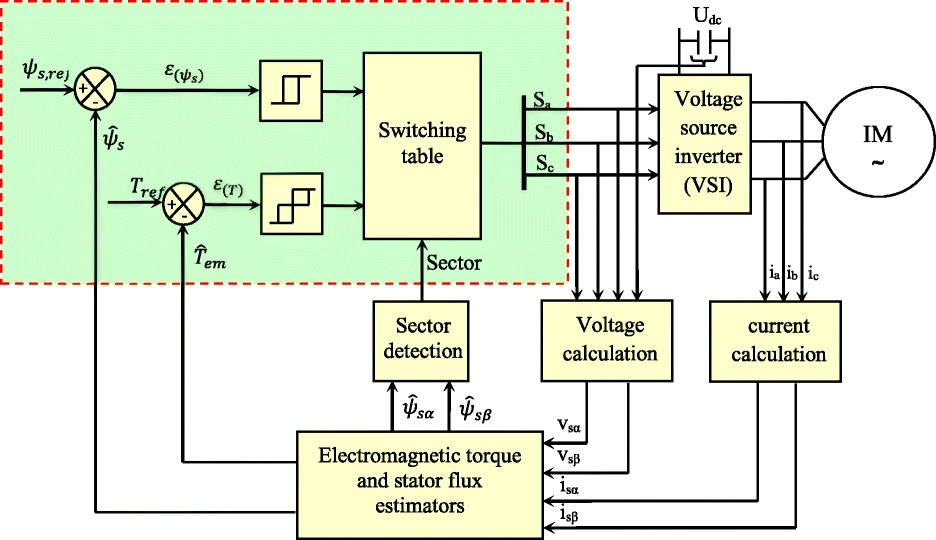
\includegraphics[width=0.8\textwidth]{Figures/dtc_schema.jpg}
	\caption[Direct Torque Control - from~\citet{Quanjli:DTC_schema:2019}.]{Direct Torque Control - from~\citet{Quanjli:DTC_schema:2019}.}
	\label{fig:example_DTC} %chktex 24
\end{figure}
Note that the nature of only switching vectors when the hysteresis is surpassed results in a variable switching frequency as opposed to \gls{foc} that has a fixed switching frequency. Another feature of the \gls{dtc} is that it does not need any modulators, as it directly chooses the voltage vector to be applied.

 \gls{dtc} is a very accessible method, with simpler implementation than \gls{foc} a faster dynamic response and low sensitivity to motor parameters, but it falls short in steady state operation with torque and current ripple often bigger than its rival \gls{foc}~\cite{Zhong:DTC_pmsm_dynamics:1997,Niu:DTC_vs_other_DTC_vs_FOC:2016}.



\subsection{Model Predictive Control}
With the increase in computational power, the \gls{mpc} has gained space among the machine controllers as it handles multivariable non-linear cases, is easy to integrate constraints, and has a great dynamic response and integrates constraint managing~\cite{Vazquez:MPC_uses:2014}. The model predictive controller's basic idea is to use a mathematical model of the controlled system to test several control actions and make a prediction about the system response. This prediction is then evaluated by a cost function that can include some soft constraints and the control action with the smaller cost is chosen as optimal.~\citet{Vazquez:MPC_in_power_systems_review:2017:IEEE} classifies the topologies typically used in power converters and drives into continuous set, and finite set, based on the process used to find the optimal control. 

Continuous set is very similar to predictive controllers used on other control fields, it computes a continuous control signal and uses a modulator to generate these voltage vectors. This topology comes with the advantage of fixed switching frequency at the cost of harder implementation and processing power requirements, as it needs an optimization solver. The finite set topology explores the limited control options of power converters to simplify the optimization process. This topology tests a set of the possible control vectors (this set can contain all or part of the possible vectors), and evaluates each of the vectors based on the predictions. While simpler to formulate, this method results in the chosen vector being applied to the full switching period, which results in a higher ripple when compared with a strategy that uses a modulator at the same control frequency. Another property of this strategy is the variable switching frequency, as the same vector can be chosen consecutively. 

To reduce the problem of applying the vector for the full timestep, a subset of finite set topology was presented. It adds time as part of the equation by computing the optimal switching sequence instead of the optimal switching vector, similar to a modulator~\cite{Vazquez:MPC_in_power_systems_review:2017:IEEE}. This allows the controller to choose a set of vectors to be switched in a given sequence with a duration also chosen by the controller.

When applied to \gls{pmsm} the predictive controllers are commonly designed with the dq0 model \Cref{eq:motor_with_inductances_no_derivative}~\cite{Sun:MPC_deadbeat_PMSM:2021}, and may track the currents or the torque to a given reference. The current tracking computational cost tends to be lower as the current optimization can be done offline while tracking torque makes online parameter estimation easier. If the topology is chosen to be continuous, a solver needs to be designed, one of the approaches is to expand the model and cost function into Taylor series approximations, and then use the derivative of the cost function to create a control law~\cite{Errouissi:MPC_taylor_series:2012}. 
% The main issues with developing an \gls{mpc} are to correctly model the system, proper cost function design, and manage computational cost to enable implementation,